\documentclass{beamer}

\usepackage{multicol}
\usepackage{listings}
\usepackage{textcomp}
\usepackage{ulem}
\usepackage{cancel}
\usepackage{tikz}
\usetikzlibrary{shapes,arrows,positioning}

\newcommand{\textapprox}{\raisebox{0.5ex}{\texttildelow}}

\lstset{ %
  backgroundcolor=\color{white},   % choose the background color
  captionpos=b,                    % sets the caption-position to bottom
  commentstyle=\color{mygreen},    % comment style
  escapeinside={\%*}{*)},          % if you want to add LaTeX within your code
  keywordstyle=\color{blue},       % keyword style
  stringstyle=\color{mymauve},     % string literal style
  showstringspaces=false,
  basicstyle=\ttfamily,
  columns=fullflexible,
  keepspaces=true,
  literate={~} {\textapprox}{1},
}

\title{A Language for the Specification and Efficient Implementation
  of Type Systems}
\author{Pascal Wittmann}
\institute{TU Darmstadt}
\date{October 23, 2014}

\begin{document}

\begin{frame}[plain]
  \titlepage{}
\end{frame}

\begin{frame}[fragile]
  \frametitle{Motivation}
\begin{example}{Simply typed lambda calculus + Subtyping}
  \begin{lstlisting}

~S = ~T
======== S-refl
~S <: ~T

~T1 <: ~S1
~S2 <: ~T2    
======================== S-arrow 
~S1 -> ~S2 <: ~T1 -> ~T2
  \end{lstlisting}
\end{example}
\end{frame}

\begin{frame}[fragile]
  \frametitle{Optimization Strategies}
  \begin{itemize}
  \item<1-> Unfold typing rules
\begin{lstlisting}
Int = Int           ~A -> ~B = Int 
========== R1       =============== R2
Int <: Int          ~A -> ~B <: Int
\end{lstlisting}
\begin{lstlisting}
Int = ~C -> ~D      ~A -> ~B = ~C -> ~D
=============== R3  ==================== R4
Int <: ~C -> ~D     ~A -> ~B <: ~C -> ~D
\end{lstlisting}
  \item<2-> Remove typing rules that are subsumed by other typing
    rules
    \begin{align*}
      \text{\texttt{\textapprox A -> \textapprox B = \textapprox C ->
          \textapprox D}} &\implies (\text{\texttt{\textapprox T1
          <:\textapprox S1}} \land \text{\texttt{\textapprox S2 <:\textapprox T2}}) \\
      (\text{\texttt{\textapprox T1 <:\textapprox S1}} \land
      \text{\texttt{\textapprox S2 <:\textapprox T2}})
      &\implies \text{\texttt{\textapprox A -> \textapprox B =
          \textapprox C -> \textapprox D}} 
    \end{align*}
  \end{itemize}
\end{frame}

\begin{frame}[fragile]
\frametitle{Optimization Strategies}
\begin{itemize}
\item<1-> Removal of typing rules with unsatisfiable premises
\begin{multicols}{2}
\begin{lstlisting}
~A -> ~B = Int
=============== R2
~A -> ~B <: Int
\end{lstlisting}
\begin{lstlisting}
Int = ~C -> ~D
=============== R3
Int <: ~C -> ~D
\end{lstlisting}
\end{multicols}
\item<2-> Removal of valid premises
\begin{lstlisting}
Int = Int
========== R1
Int <: Int
\end{lstlisting}
\item<3-> After optimizations we have the following typing rules
\begin{lstlisting}
                ~T1 <: ~S1 
                ~S2 <: ~T2    
========== R1   ======================== S-arrow 
Int <: Int      ~S1 -> ~S2 <: ~T1 -> ~T2
\end{lstlisting}
\end{itemize}
\end{frame}

\begin{frame}
  \frametitle{Architecture}
  \begin{itemize}
  \item Automatic translation of specifications into first-order formulas
  \item Automated theorem provers are used to validate applicability
    of optimizations
  \item Generation of a type checker from optimized specifications
  \end{itemize}
  \vspace{.8cm}
  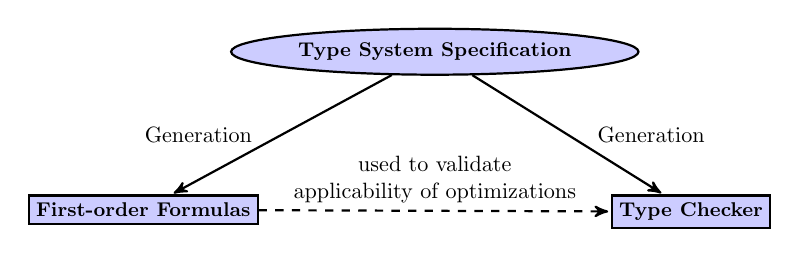
\begin{tikzpicture}[scale=.8,transform shape,->,>=stealth',shorten >=1pt,auto,align=center,node distance=1cm,thick,main node/.style={fill=blue!20,rectangle,draw,font=\small\bfseries}]
    \node[main node, style={ellipse}] (1) {Type System Specification};
    \node[main node] (2) [below left=2cm and .5cm of 1]  {First-order Formulas};
    \node[main node] (3) [below right=2cm and .5cm of 1] {Type Checker};

  \path[every node/.style={}]
  (1) edge node [outer sep=10pt,left] {Generation} (2)
  (1) edge node [outer sep=10pt,right] {Generation} (3);

  \path[every node/.style={}, dashed]
  (2) edge node [above] {used to validate \\ applicability of
    optimizations} (3);
  \end{tikzpicture}
\end{frame}

\begin{frame}
  \frametitle{Type Checker}
  \begin{itemize}
  \item Translation of typing rules in normalized templates
%    \begin{itemize}
%    \item no implicit equalities
%    \item explicit premise dependencies
%    \end{itemize}
  \item Optimization of templates
  \item Type checking according to templates using a generic type
    checker
  \end{itemize}
\vspace{.5cm}
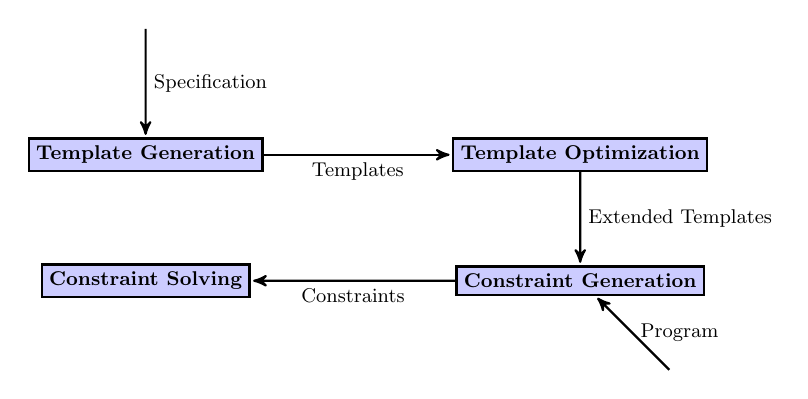
\begin{tikzpicture}[scale=.8,transform shape,->,>=stealth',shorten >=1pt,auto,align=center,node distance=2cm,
  thick,main node/.style={rectangle,fill=blue!20,draw,font=\small\bfseries}]
  \node[main node] (1) {Template Generation};
  \node[main node] (2) [right=3cm of 1] {Template Optimization};
  \node[main node] (3) [below of=2] {Constraint Generation};
  \node[main node] (4) [below of=1] {Constraint Solving};
  \coordinate [below right of=3] (5);
  \coordinate [above of=1] (6);

  \path[every node/.style={font=\small}]
    (1) edge node [right, below] {Templates} (2)
    (2) edge node [right] {Extended Templates} (3)
    (5) edge node [right] {Program} (3)
    (3) edge node [right, below] {Constraints} (4)
    (6) edge node [right] {Specification} (1);
\end{tikzpicture}
\end{frame}

\begin{frame}
  \frametitle{Conclusion \& Future Work}
  \begin{itemize}
  \item We contribute
    \begin{itemize}
    \item a declarative, high-level specification language for type
      system
    \item a translation of specifications into first-order formulas
    \item optimization strategies to reduce the need of backtracking
      in the type checker
    \item a type checker generator, which generates constraint-based
      type checkers
    \end{itemize}
  \item We plan to
    \begin{itemize}
    \item develop more optimization strategies (e.g.\ to optimize
      subsumption-like rules)
    \item develop heuristics and proof strategies to validate the
      applicability of optimizations
    \item apply our work to more realistic programming languages
    \end{itemize}
  \end{itemize}
\end{frame}

\end{document}